%% ========================================================================
%%%% Document settings
%% ========================================================================

%% How to separate paragraphs: indention ("no") or spacing ("half", "full",
%% ...).
\newcommand{\myparskip}{half}

%% Inner binding correction. This value depends on the method which is
%% being used to bind your printed result. Some techniques do not
%% require a binding correction at all ("0mm"), other require for
%% example "5mm". Refer to KOMA script documentation for a detailed
%% explanation what a binding correction is and how to measure it.
\newcommand{\myBCOR}{0mm}

%% Either you are creating a document which is printed on both, left pages and right pages (twoside) or you create a document which is printed on right pages only (oneside).
%% e.g. "true" or "false"
\newcommand{\mytwoside}{false}

%% Color of the headings and so forth in RGB (red,green,blue) values.
%% e.g. "30,103,182" (blue/turquois), "0,0,0" (black), ...
\newcommand{\mydispositioncolor}{0,0,0}%{22,72,154}

%% Line spacing in %/100. For example 1.5 means 150% of the usual line spacing. Please use with caution: 100% ("1.0") is fine because the font was designed for it.
%% e.g. 1.0, 1.5, 2.0
\newcommand{\mylinespread}{1.5}

\newcommand{\mycolorlinks}{false}  %% "true" or "false"
%% Enables or disables colored links (hyperref package).
% turn on/off colored links (on: better for on-screen reading; 
                            %off: better for printout versions)

%% See babel documentation for further details.
%% NOTE: The *last* language is the active one!
%% "english,ngerman", "ngerman,english", ...
\newcommand{\mylanguage}{english,ngerman}

%% ========================================================================
%%%% Document metadata
%% ========================================================================

%% Student:
\newcommand{\myauthor}{Jonathan Diebel, Jannis Kaniaros und Dario Nieddu}
\newcommand{\myhomestreet}{}
\newcommand{\myhomepostalnumber}{}
\newcommand{\myhometown}{}
\newcommand{\myid}{9883850, 5934448, }

%% Titel und PDF-Einstellungen
\newcommand{\myworktype}{Ausarbeitung}
\newcommand{\myworktitle}{}
\newcommand{\mytitle}{Cucina intelligente di Massimo}
\newcommand{\mysubtitle}{Intelligent Agent Systems}
\newcommand{\mysubject}{}
\newcommand{\mykeywords}{}

%% nur bei Bachelorarbeit wichtig: Art des Abschlusses:
\newcommand{\mydegree}{Master of Science}

%% Dualer Partner
\newcommand{\mydualpartner}{}
\newcommand{\mydualpartnerLocation}{}
\newcommand{\mysupervisor}{}

%% Duale Hochschule
\newcommand{\myuniversity}{Center for Advanced Studies der\\Dualen Hochschule Baden-Württemberg}
\newcommand{\mycourse}{T3M40501}
\newcommand{\mystudy}{}
\newcommand{\myevaluator}{Prof. Dr. Nathan Sudermann-Merx}

%% Datum
\newcommand{\mysubmissionday}{31}
\newcommand{\mysubmissionmonth}{März}
\newcommand{\mysubmissionyear}{2025}

\newcommand{\myprocessingperiodbegin}{}
\newcommand{\myprocessingperiodend}{}

%% ========================================================================
%%%% Other settings
%% ========================================================================

%% !!FIRST!! Load preamble
\documentclass[
   fontsize=12pt,      %% size of the main text
   parskip=\myparskip, %% vertical space between paragraphs (instead of indenting first par-line)
   DIV=calc,           %% calculates a good DIV value for type area; 66 characters/line is great
   headinclude=true,   %% is header part of margin space or part of page content?
   footinclude=false,  %% is footer part of margin space or part of page content?
   open=right,         %% "right" or "left": start new chapter on right or left page
   appendixprefix=true,%% adds appendix prefix; only for book-classes with \backmatter
   bibliography=totoc, %% adds the bibliography to table of contents (without number)
   numbers=noenddot,   %% remove dot after the chapter / section number
   BCOR=\myBCOR,       %% binding correction (depends on how you bind the resulting printout.
   twoside=\mytwoside       %% oneside: document is not printed on left and right sides, only right side 
                       %% twoside: document is printed on left and right sides
]{scrbook}

% set raggedbottom if \mytwoside is 'true' to prevent weird spaces between text blocks
\makeatletter
\if@twoside%
   \raggedbottom
\fi%  
\makeatother

%% Set paper and border size
\usepackage[paper=a4paper,left=25mm,right=25mm,top=25mm,bottom=25mm]{geometry}

%% UTF8 as input characters; UCS incompatible to biblatex
\usepackage[utf8]{inputenc}

%% The default setting of the language is American. Please change settings for
%% additional or alternative languages used in main.tex.
%% Please note that the default language of the document is the *last* language
%% which is added to the package options.
%% To set only parts of your document in a different language as the rest,
%% use for example\newline\verb+\foreignlanguage{ngerman}{Beispieltext in deutscher Sprache}+\newline
\usepackage[\mylanguage]{babel}

%% This package defines basic colors. If you want to get rid of colored links
%% and headings please change corresponding value in main.tex to {0,0,0}.
%% Used for links and so forth in screen-version
\usepackage[dvipsnames]{xcolor}
\definecolor{DispositionColor}{RGB}{\mydispositioncolor}

%% The widely used package to use graphical images within a LaTeX document.
%% \includegraphics[width=42mm]{figures/image}
\usepackage[pdftex]{graphicx}

%% For example on title pages you might want to have a logo on the upper right
%% corner of the first page (only). The package \texttt{eso-pic} is able to
%% place things on absolute and relative positions on the whole page.
\usepackage{eso-pic}

%% Inline enumerations
\usepackage[inline]{enumitem}

%% List of abbreviations
\usepackage[printonlyused]{acronym}

%% Use biblatex for bibliography
%% With "Sorting=None" the numbering is done according to the order of appearance. 
\usepackage[backend=biber,style=apa,sorting=none]{biblatex}

%% Used for quotes
\usepackage{csquotes}

%% Add fontec to hyphenate umlaut and fix-cm to fix changes in section heading
\usepackage[T1]{fontenc}
\usepackage{fix-cm}

%% Add default bibliography
\addbibresource{etc/literature.bib}

%% Give name to bibliography
% \bibliography{Quellenverzeichnis}

%% ========================================================================
%%%% Typographic settings
%% ========================================================================

%% If you have to enlarge the distance between two lines of text, you can
%% increase it using the \texttt{\mylinespread} command in \texttt{main.tex}. By default, it is
%% deactivated (set to 100~percent). Modify only with caution since it influences the
%% page layout and could lead to ugly looking documents.
\linespread{\mylinespread}

\renewcommand*{\chapterheadstartvskip}{\vspace*{0\baselineskip}}% Abstand einstellen

%% Reduce space between section and chapter headings
\RedeclareSectionCommand[
   beforeskip=0pt,
   afterskip=1sp
]{chapter}

\RedeclareSectionCommand[
   beforeskip=0pt,
   afterskip=1sp
]{section}

\RedeclareSectionCommand[
   beforeskip=0pt,
   afterskip=1sp
]{subsection}

\RedeclareSectionCommand[
   beforeskip=0pt,
   afterskip=1sp
]{subsubsection}

%% This document template is able to generate an output that uses colorized
%% headings, captions, page numbers, and links. The color named
%% `DispositionColor' used in this document is defined near the definition
%% of package xcolor
%% The changes required for headings, page numbers and captions are defined
%% here.
%% Settings for colored links are handled by the definitions of the
%% hyperref package
% \setheadsepline{.4pt}[\color{DispositionColor}]
% \renewcommand{\headfont}{\normalfont\rmfamily\color{DispositionColor}}
% \renewcommand{\pnumfont}{\normalfont\rmfamily\color{DispositionColor}}
% \addtokomafont{disposition}{\color{DispositionColor}}
% \addtokomafont{caption}{\color{DispositionColor}\footnotesize}
% \addtokomafont{captionlabel}{\color{DispositionColor}}


%% Add package to add long text tables
\usepackage{longtable}

%% ========================================================================
%%%% Source code highlighting
%% ========================================================================

%% Minted for source code highlighting
\usepackage[newfloat]{minted}
\removefromtoclist[float]{lol}% must be after loading `minted`.

%%\BeforeBeginEnvironment{minted}{\medskip}
%%\AfterEndEnvironment{minted}{\smallskip}

%% XColor for color definitions
\usepackage{xcolor}

%% Define background color for style "friendly"
\definecolor{friendlybg}{HTML}{f0f0f0}

%% Settings for source code
\definecolor{codebg}{rgb}{0.95,0.95,0.95}
\setminted{
   bgcolor=codebg,
   startinline=true,
   obeytabs=true,
   tabsize=4,
   %linenos,
   breaklines,
   fontsize=\small,
   baselinestretch=1.2,
   samepage=true
}

\renewcommand{\listingname}{Listing}

\usepackage{etoolbox}

\makeatletter
\AtBeginEnvironment{minted}{\dontdofcolorbox}
\def\dontdofcolorbox{\renewcommand\fcolorbox[4][]{##4}}
\makeatother

%% Use caption package to customize image, code and table captions
\usepackage[
   font =      {footnotesize, sf}, %% Sans Serif font family
   labelfont = {footnotesize, bf} %% Bold font series
]{caption}

%% for the code-block environment with listing and reference possibility:
%% \begin{code}{<language>}{<caption>}{<label>} 
%% ... 
%% \end{code}
%% is also used with listings so there is a list of code blocks
\usepackage{listings}
\usepackage[figure,table,lstlisting]{totalcount}
\renewcommand{\lstlistingname}{Listing}
\captionsetup[lstlisting]{skip=5pt,belowskip=15pt} % spacing for the label
% %% the following see also here: https://github.com/gpoore/minted/issues/108
\newcommand{\storeCaption}{}
\newcommand{\storeLabel}{}
\newenvironment{codelisting}{\captionsetup{type=lstlisting}}{}
\newenvironment{code}[3]
{%
   \VerbatimEnvironment
   \renewcommand{\storeCaption}{#2}%
   \renewcommand{\storeLabel}{#3}%
   \begin{minipage}{\linewidth}%
      \begin{codelisting}%
         \begin{minted}{#1}%
	}
	{%
	\end{minted}%
         \caption{%
            {
                  \setmintedinline{fontsize=\footnotesize}%
                  \storeCaption %
               }%
         }%
         \label{\storeLabel}%
      \end{codelisting}%
   \end{minipage}%
}


% New commands for text sub- and superscript
\let\tsup\textsuperscript
\let\tsub\textsubscript

% Subfigures
\usepackage{subcaption}

% Color boxes
\usepackage[most]{tcolorbox}

% Math
\usepackage{amsmath}

%% LoF & LoL indentation
\usepackage[titles]{tocloft}
\cftsetindents{fig}{0pt}{2.3em}
\makeatletter
\renewcommand{\l@figure}{\@dottedtocline{1}{0em}{2.3em}}
\renewcommand{\l@lstlisting}{\@dottedtocline{1}{0em}{2.3em}}
\makeatother
% \cftsetindents{code}{0pt}{2.3em}

%% TikZ / Plots
% \usepackage{tikzit}
% \usepackage[edges]{forest}
% \usetikzlibrary{arrows.meta}
\usepackage{pgfplots}
\pgfplotsset{compat=1.18}
\usepgfplotslibrary{statistics}

%% Autoref command capitalizing the first letter (English only)
\newcommand{\Autoref}[1]{%
   \begingroup%
   \def\chapterautorefname{Chapter}%
   \def\sectionautorefname{Section}%
   \def\subsectionautorefname{Subsection}%
   \def\subsubsectionautorefname{Subsubsection}%
   \def\paragraphautorefname{Paragraph}%
   \def\tableautorefname{Table}%
   \def\equationautorefname{Equation}%
  \autoref{#1}%
  \endgroup%
}

\hyphenation{ab-hör-si-cher-en Funk-ti-ons-um-fang Bild-er-ken-nung}

%% !!LAST!! Do PDF settings
%% ========================================================================
%%%% PDF settings
%% ========================================================================

\pdfcompresslevel=9

%% Declarations of hyperref should be the last definitions of the preamble
\usepackage[
    unicode=true,
    backref,
    pagebackref=false,
    bookmarks=true,
    bookmarksopen=false,
    pdfpagemode=UseNone,
    plainpages=false,
    urlcolor=DispositionColor,
    linkcolor=DispositionColor,
    citecolor=DispositionColor,
    anchorcolor=DispositionColor,
    colorlinks=\mycolorlinks,
    breaklinks
]{hyperref}

%% all strings need to be loaded after hyperref was loaded with unicode support
%% if not the field is garbled in the output for characters like ČŽĆŠĐ
\hypersetup{
    pdftitle = {\mytitle},
    pdfauthor = {\myauthor},
    pdfsubject = {\mysubject},
    pdfproducer = {\myauthor},
    pdfkeywords = {\mykeywords}
}

%% Break URLs in bibliography
\PassOptionsToPackage{hyphens}{url}
\setcounter{biburllcpenalty}{8000}

%% ========================================================================
%%%% begin{document}
%% ========================================================================
\begin{document}
\rmfamily
\frontmatter
%% Big roman page numbering
\pagenumbering{Roman}

%% Titelseite
%% Verwendung von Studienarbeit-Deckblatt
%% ========================================================================
%%%% Information
%% ========================================================================
%% Titelseite für Arbeiten mit der dualen Hochschule Mosbach.
%% Die anzuzeigenden Daten werden in der Datei main.tex festgelegt.

\begin{titlepage}
    
    %% University Logo
    \AddToShipoutPicture*{
        \AtPageUpperLeft{
            \hspace{\paperwidth}
            \raisebox{-52mm}{
                \makebox[-39mm][r]{
\includegraphics{template/figures/University_Logo_CAS}}
            }
        }
    }

    \begin{center}
        ~
        \vfill\vfill\vfill \vfill\vfill

        % \sffamily

        {\LARGE\bfseries\mytitle}

        {\large\mysubtitle}

        \vfill\vfill
        {\normalsize\bfseries\myworktype}\\

        \vfill \vfill
        für das % For the \mystudy ~Department at the\\
        {\normalsize\bfseries\myuniversity}

        \vfill
        von\\
        \myauthor

        \vfill
        \mysubmissionday.~\mysubmissionmonth ~\mysubmissionyear

        \vfill\vfill\vfill
    \end{center}

    \rmfamily{
        \begin{tabular}{ll}
            % Processing period     & \myprocessingperiodbegin ~- \myprocessingperiodend \\
            Matrikelnummern            & \myid                                              \\
            Kurs                & \mycourse                                          \\
            Dozenten & \myevaluator                                       \\
        \end{tabular}
    }

\end{titlepage}

\newpage

%% Verwendung von Projekt-Deckblatt
% %% ========================================================================
%%%% Information
%% ========================================================================
%% Titelseite für Arbeiten mit der dualen Hochschule Mosbach und der AUDI AG.
%% Die anzuzeigenden Daten werden in der Datei main.tex festgelegt.

\begin{titlepage}

    %% Company Logo
    \AddToShipoutPicture*{
        \AtPageUpperLeft{
            \hspace{\paperwidth}
            \raisebox{-50mm}{
                \makebox[-129mm][r]{
\includegraphics[width=42mm]{template/figures/University_Logo.png}}
            }
        }
    }

    %% University Logo
    \AddToShipoutPicture*{
        \AtPageUpperLeft{
            \hspace{\paperwidth}
            \raisebox{-52mm}{
                \makebox[-39mm][r]{
\includegraphics[width=42mm]{template/figures/Company_Logo.png}}
            }
        }
    }

    \begin{center}
        ~
        \vfill\vfill\vfill \vfill\vfill

        \sffamily

        {\LARGE\bfseries\mytitle}

        {\large\mysubtitle}

        \vfill\vfill
        {\normalsize\bfseries\myworktype~\myworktitle}\\

        \vfill \vfill
        Im Studiengang \mystudy\\
        an der \myuniversity

        \vfill
        von\\
        \textbf{\myauthor}

        \vfill
        \mysubmissionday. \mysubmissionmonth~\mysubmissionyear

        \vfill\vfill\vfill
    \end{center}

    \sffamily{
        \begin{tabular}{ll}
            Matrikelnummer                & \myid                  \\
            Ausbildungsfirma              & \mydualpartner         \\
                                          & \mydualpartnerLocation \\
            Betreuer der Ausbildungsfirma & \mysupervisor          \\
        \end{tabular}
    }

\end{titlepage}

\newpage

%% Verwendung von Bachelor-Deckblatt
% %% ========================================================================
%%%% Information
%% ========================================================================
%% Titelseite für Arbeiten mit der dualen Hochschule Mosbach und der AUDI AG.
%% Die anzuzeigenden Daten werden in der Datei main.tex festgelegt.

\begin{titlepage}

    %% Company Logo
    \AddToShipoutPicture*{
        \AtPageUpperLeft{
            \hspace{\paperwidth}
            \raisebox{-50mm}{
                \makebox[-136mm][r]{
\includegraphics[width=42mm]{template/figures/Company_Logo.png}}
            }
        }
    }

    %% University Logo
    \AddToShipoutPicture*{
        \AtPageUpperLeft{
            \hspace{\paperwidth}
            \raisebox{-52mm}{
                \makebox[-31mm][r]{
\includegraphics[width=42mm]{template/figures/University_Logo.png}}
            }
        }
    }

    \begin{center}
        ~
        \vfill\vfill\vfill \vfill\vfill

        % \sffamily

        {\LARGE\bfseries\mytitle}

        {\large\mysubtitle}

        \vfill\vfill
        {\normalsize\bfseries\ BACHELORARBEIT}\\

        \vfill\vfill
        für die Prüfung zum \\
        \mydegree

        \vfill
        im Studiengang \mystudy\\
        an der \myuniversity

        \vfill
        von\\
        \textbf{\myauthor}

        \vfill
        \mysubmissionday. \mysubmissionmonth~\mysubmissionyear

        \vfill\vfill\vfill
    \end{center}

    \rmfamily{
        \begin{tabular}{ll}
            Bearbeitungszeitraum            & \myprocessingperiodbegin~--~\myprocessingperiodend \\
            Matrikelnummer, Kurs            & \myid, \mycourse                       \\
            Ausbildungsfirma                & \mydualpartner, \mydualpartnerLocation \\
            Betreuer der Ausbildungsfirma   & \mysupervisor                          \\
            Gutachter der Dualen Hochschule & \myevaluator
        \end{tabular}
    }

\end{titlepage}

\newpage


%% Sperrvermerk
% %% Sperrvermerk
\chapter*{Sperrvermerk}
\thispagestyle{empty}
Die vorliegende \myworktype ~mit dem Titel \enquote{\emph{{\mytitle}}} basiert auf internen, vertraulichen Daten und Informationen des Unternehmens \mydualpartner.

Sie darf nur dem Erst- und Zweitgutachter sowie befugten Mitgliedern der Prüfungsorgane zugänglich gemacht werden. Eine Veröffentlichung und Vervielfältigung ist -- auch in Auszügen -- nicht gestattet.

Eine Einsichtnahme durch Unbefugte bedarf einer schriftlichen Genehmigung durch den Verfasser und das Unternehmen.

\newpage
%% Eidesstattliche Erklärung
% %% Neuen Befehl für Textfelder definieren
\newcommand{\textfield}[2]{
    \vbox{
        \hsize=#1\kern3cm\hrule\kern1ex
        \hbox to \hsize{\strut\hfil\footnotesize#2\hfil}
    }
}

%% Ehrenwörtliche Erklärung
\chapter*{Ehrenwörtliche Erklärung}
Wir versichern hiermit, dass wir unser \myworktype ~mit dem Thema: \enquote{\emph{{\mytitle}}} selbstständig verfasst und keine anderen als die angegebenen Quellen und Hilfsmittel benutzt haben.

% Ich versichere zudem, dass die eingereichte elektronische Fassung mit der gedruckten Fassung übereinstimmt.\\
%% Ort, Datum und Unterschrift
\hbox to \hsize{\textfield{6cm}{Ort, Datum}\hfil\hfil\textfield{6cm}{Jan-Patrick Hespelt}}
\hbox to \hsize{\textfield{6cm}{Ort, Datum}\hfil\hfil\textfield{6cm}{Jannis Kaniaros}}
\hbox to \hsize{\textfield{6cm}{Ort, Datum}\hfil\hfil\textfield{6cm}{Jonas Landwehr}}


\newpage

%% Abstract
% %% ---------------------------------------------
%% Kurzfassung
%% ---------------------------------------------
\chapter*{Kurzfassung} \label{chap:Kurzfassung}
\thispagestyle{plain}
Kurzfassung Deutsch

\cleardoublepage
%% ---------------------------------------------
%% Abstract
%% ---------------------------------------------
% \begingroup
%% Group for removing the page break
% \renewcommand{\cleardoublepage}{}
% \renewcommand{\clearpage}{}
\chapter*{Abstract} \label{chap:abstract}
\thispagestyle{plain}
% \endgroup
Kurzfassung Englisch

%% Inhaltsverzeichnis
%% Rename contents
% \renewcommand{\contentsname}{Table of Contents}
\tableofcontents
\newpage

%% Abkürzungen
\chapter{Abkürzungsverzeichnis}
\begin{acronym}[CRISP-DM] % longest acronym defines length
    \acro{crisp}[CRISP-DM]{Cross-Industry Standard Process for Data Mining}

    \acro{db}[DB]{Datenbank}
    \acroplural{db}[DBs]{Datenbanken}

    \acro{iot}[IoT]{Internet of Things}

    \acro{llm}[LLM]{Large Language Model}
    \acro{ml}[ML]{Machine Learning}

    \acro{pos}[POS]{Part of Speech}
\end{acronym}

%% Abbildungsverzeichnis anzeigen, wenn Abbildungen in Dokument enthalten sind
\iftotalfigures
    \cleardoublepage
    \phantomsection
    \addcontentsline{toc}{chapter}{\listfigurename}
    \listoffigures
\fi

%% Tabellenverzeichnis anzeigen, wenn Tabellen in Dokument enthalten sind
\iftotaltables
    \cleardoublepage
    \phantomsection
    \addcontentsline{toc}{chapter}{\listtablename}
    \listoftables
\fi

%% Code-Verzeichnis anzeigen, wenn Code-Blöcke in Dokument enthalten sind
\renewcommand\lstlistlistingname{Codeverzeichnis}
\iftotallstlistings
    \cleardoublepage
    \phantomsection
    \addcontentsline{toc}{chapter}{\lstlistlistingname}
    \lstlistoflistings
\fi

%% Gender Disclaimer
% %% Gender-Hinweis
\cleardoublepage

\chapter*{Gender-Hinweis}
\thispagestyle{plain}

Aus Gründen der besseren Lesbarkeit wird in dieser \myworktype ~bei Personenbezeichnungen und personenbezogenen Hauptwörtern die männliche Form verwendet. Entsprechende Begriffe gelten im Sinne der Gleichbehandlung grundsätzlich für alle Geschlechter. Die verkürzte Sprachform hat nur redaktionelle Gründe und beinhaltet keine Wertung.

\newpage

%% Marks main part using Arabic page numbers and such; Only available in scrbook
\mainmatter

\pagenumbering{arabic}
%% Add new chapters here
%!TEX root = ../main.tex

\chapter{Einleitung}
\label{chap:einleitung}

Restaurants sind Orte, an denen Menschen nicht nur gutes Essen genießen, sondern auch eine Auszeit vom Alltag nehmen können. Ob für ein romantisches Dinner, ein schnelles Mittagessen oder ein entspanntes Treffen mit Freunden – die Gastronomie bietet für jeden Anlass das passende Ambiente. Doch in einer Welt, die immer schneller wird und in der Zeit oft zur kostbarsten Ressource wird, stehen auch Restaurants vor der Herausforderung, sich an die Bedürfnisse ihrer Gäste anzupassen.

Ein neues Konzept revolutioniert nun das Restauranterlebnis: Kunden können bereits beim Betreten des Restaurants oder bei der Reservierung angeben, wie viel Zeit sie für ihren Besuch einplanen. Ob 30 Minuten für eine schnelle Mahlzeit oder zwei Stunden für ein ausgedehntes Dinner – dieses innovative Modell ermöglicht es, den Service individuell auf die Wünsche der Gäste abzustimmen. So wird nicht nur die Effizienz gesteigert, sondern auch das Restauranterlebnis persönlicher und flexibler gestaltet.

In dieser Arbeit wird das Konzept der zeitbasierten Reservierung genauer untersucht und ein optimiertes intelligentes Mutliagentensystem vorgestellt, das die Umsetzung in einem Restaurant, der \emph{Cucina intelligente di Massimo}, unterstützt.

\begin{figure}[h]
    \centering
    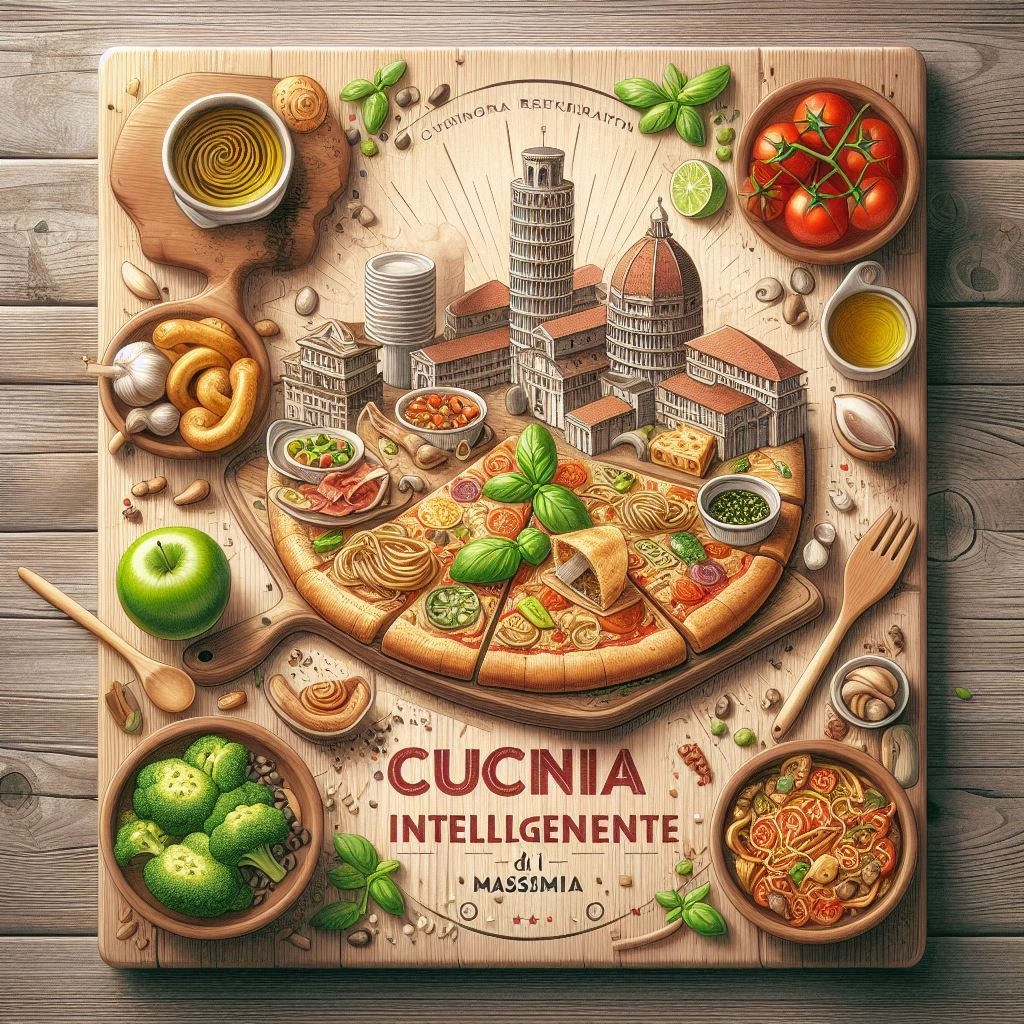
\includegraphics[width=0.5\textwidth]{img/cover.jpg}
    \caption{Cover}
    \label{fig:cover}
\end{figure}

% Im Folgenden werden die Anforderungen an das System analysiert, die Architektur und die Funktionsweise des Systems beschrieben und die Implementierung sowie die Evaluation des Systems vorgestellt. Abschließend werden die Ergebnisse zusammengefasst und ein Ausblick auf mögliche Erweiterungen gegeben.
%!TEX root = ../main.tex

\chapter{Design}
\label{chap:design}

\section{Agenten}
\label{sec:agenten}

Im Modell werden drei verschiedene Agenten eingesetzt: \emph{Customer Agents}, \emph{Service Agents} sowie ein \emph{Manager Agent}. Die Agenten sind in einem Multi-Agenten-System organisiert, in dem sie miteinander kommunizieren und sich gegenseitig beeinflussen.

\subsection{Customer Agents}
\label{subsec:customer_agents}
Customer Agents beschreiben eine Gruppe von Kunden, die ein Restaurant besuchen und eine Bestellung aufgeben wollen. Die Attribute der Agenten werden größtenteils randomisiert generiert. Dazu zählen die genaue Anzahl der Personen, die maximale Wartezeit sowie das ausgewählte Gericht.

Die Agenten werden über einen internen Status gesteuert, der den aktuellen Zustand des Agenten beschreibt. Die möglichen Zustände sind \emph{Waiting for Service Agent}, \emph{Waiting for food}, \emph{Eating}, \emph{Finished Eating}, \emph{Rejected} und \emph{Done}. Der Status wird durch die verschiedenen Aktionen des Agenten verändert. 

Wichtig im Zuge dieses Konzepts ist, dass die Agenten das Restaurant nicht verlassen, sobald ihre Zeit abgelaufen ist. Stattdessen wird das Essen beendet, dafür sinkt jedoch die Bewertung.

Wenn die Customer Agents ihr Essen beendet haben, geben sie eine Bewertung ab. Diese Bewertung ist eine Funktion mit mehreren Zufallsfaktoren:

\begin{equation*}
    r = \text{round}\left(\max\left(r_{\text{min}}, \min\left(r_{\text{max}}, r_{\text{max}} - \alpha \cdot \text{exceedance} - \beta \cdot \text{error} + \gamma\right)\right), 2\right)
\end{equation*}

wobei:
\begin{itemize}
    \item $r$ die finale Bewertung ist,
    \item $r_{\text{min}}$ die minimal mögliche Bewertung ist,
    \item $r_{\text{max}}$ die maximal mögliche Bewertung ist,
    \item $\alpha$ die Gewichtung der Wartezeitstrafe ist,
    \item $exceedance$ der Quotient aus der tatsächlichen Wartezeit und der angegebenen maximalen Zeit ist (nur bei Überschreitung, sonst 0),
    \item $\beta$ die Gewichtung für fehlerhafte Bestellungen ist,
    \item $error$ eine zufällige Fehlerquote ist,
    \item $\gamma$ eine zufällige Bewertungsvariabilität abhängig von der Gruppengröße ist.
\end{itemize}

Wird ein Kunde abgewiesen, gibt er immer die niedrigste Bewertung ab.

Im \emph{PEAS-Framework} lassen sich die Customer Agents wie folgt beschreiben:
\begin{description}
    \item[Performance Measure] Einhaltung der maximalen Zeit
    \item[Environment] Das Restaurant, Service Agents
    \item[Actuators] Bestellung aufgeben, Essen bewerten
    \item[Sensors] Wartezeit, interner Status
\end{description}

Bei den Customer Agents handelt es sich gemäß des \emph{AIMA-Framework}s um \emph{Simple Reflex Agents}, da sie ihre Aktionen basierend auf dem aktuellen Zustand und den wahrgenommenen Informationen ausführen, ohne eine interne Zustandsrepräsentation der Welt zu verwenden. Sie reagieren direkt auf die wahrgenommenen Reize, wie z.B. die erhaltene Bestellung, um ihre nächsten Aktionen zu bestimmen.


\subsection{Service Agents}
\label{subsec:service_agents}
Service Agents sind für die Bedienung der Customer Agents zuständig. Sie haben die Aufgabe, die Bestellungen der Kunden entgegenzunehmen, diese zuzubereiten und das Essen zu servieren. Jeder Service Agent hat eine Kapazität an Customer Agents, die er bedienen kann. Einmal zugewiesen, werden die Customer Agents nicht mehr von anderen Service Agents bedient, außer der Service Agent beendet seine Arbeit, dann werden seine Customer Agents an die übrigen Service Agents übergeben.

Jeder Service Agent kann pro Zeitschritt nur zwei Customer Agents bedienen, dabei wird ein Customer Agent entweder platziert oder abgewiesen und in die Status \emph{Waiting for food} bzw \emph{Rejected} versetzt, während für einen anderen Customer Agent die Zubereitung der Speisen durchgeführt wird. Da die Zubereitung der Speisen im Menü festgelegt ist und unterschiedlich lange dauert, wird deshalb entweder die Zubereitungszeit um einen Zeitschritt reduziert oder, sofern die Zubereitung abgeschlossen ist, das Essen serviert und der Customer Agent in den Status \emph{Eating} versetzt.\\
Kunden werden dann abgewiesen, wenn sie im Status \emph{Waiting for Service Agent} sind, aber die Summe aus Zubereitungs- und Essenszeit der Speisen die maximale Wartezeit überschreitet, also ein Service in der angegeben Zeit überhaupt nicht möglich ist.

Die zu bedienenden Customer Agents werden von den Service Agents in jedem Schritt dynamisch sortiert und entsprechend bedient. Dabei werden verschiedene Faktoren berücksichtigt und gewichtet, um die Interessen der Kunden (also die Minimierung der Wartezeit) sowie die Interessen des Managers (also die Maximierung des Gewinns) zu berücksichtigen.\\
Dabei wird für jeden Kunden ein Rang bestimmt - je höher der Rang, desto früher wird der Kunde bedient. Die Sortierung für neue Kunden erfolgt wie folgt:
\begin{equation*}
    r = \alpha \cdot p \cdot n + \beta \cdot \text{total\_time} + \gamma \cdot \text{time\_left}
\end{equation*}

wobei:
\begin{itemize}
    \item $r$ der Rang des Kunden ist,
    \item $p$ der Preis des Gerichts ist,
    \item $n$ die Anzahl der Personen ist,
    \item $\alpha$ die Gewichtung des Profits ist,
    \item $total\_time$ die Gesamtzeit ist, die der Kunde bereits im Restaurant verbracht hat,
    \item $\beta$ die Gewichtung der Gesamtzeit ist,
    \item $time\_left$ die verbleibende Zeit ist,
    \item $\gamma$ die Gewichtung der verbleibenden Zeit ist
\end{itemize}

Für die Sortierung der bereits im Restaurant befindlichen Kunden wird die gleiche Formel verwendet, zusätzlich jedoch noch die Zubereitungszeit der Speisen berücksichtigt wird. Damit ergibt sich folgende Formel:
\begin{equation*}
    r = \alpha \cdot p \cdot n + \beta \cdot \text{total\_time} + \gamma \cdot \text{time\_left} + \delta \cdot \text{cooking\_time}
\end{equation*}

wobei die Werte entsprechend der Formel für neue Kunden definiert sind, $cooking\_time$ die Zubereitungszeit des Gerichts und $\delta$ die Gewichtung der Zubereitungszeit ist.

Im \emph{PEAS-Framework} lassen sich die Service Agents wie folgt beschreiben:
\begin{description}
    \item[Performance Measure] Wartezeit der Kunden minimieren, möglichst hohe Bewertung, Maximierung des Gewinns
    \item[Environment] Das Restaurant, Customer Agents
    \item[Actuators] Bestellung aufnehmen, Essen zubereiten, Essen servieren, Kunden abweisen
    \item[Sensors] Neue Kunden vorhanden, Zustand der Customer Agents
\end{description}

Bei den Service Agents handelt es sich gemäß des \emph{AIMA-Framework}s ebenfalls um \emph{Simple Reflex Agents}, da sie ihre Aktionen basierend auf dem aktuellen Zustand und den wahrgenommenen Informationen ausführen, ohne eine interne Zustandsrepräsentation der Welt zu verwenden. Sie reagieren direkt auf die wahrgenommenen Reize, wie z.B. den Status der Kunden.


\subsection{Manager Agent}
\label{subsec:manager_agent}
Der Manager Agent ist für die Koordination der Service Agents zuständig. Er existiert im Restaurant nur ein Mal und hat die Aufgabe, die Service Agents zu verwalten.
%!TEX root = ../main.tex

\chapter{Mathematische Formulierung des Optimierungsproblems}
Wir haben ein engagiertes Team von Mitarbeitern und eine Reihe von Einschränkungen, die sich vor allem aus dem Arbeitsschutzgesetz ergeben. Einige Mitarbeiter arbeiten weniger Stunden und Schichten, während andere mehr arbeiten. Das muss nicht ausgewogen oder fair sein, sondern muss bestmöglich zur Zielfunktion beitragen. Die Herausforderung besteht darin, die Mitarbeiter für den nächsten Tag so einzusetzen, dass der Gesamtgewinn maximiert wird. Die Mitarbeiter werden im Laufe des Tages weder versetzt noch ausgewechselt. Darüber hinaus hat jeder Mitarbeiter einen spezifischen \mintinline{text}{customer_capacity}-Faktor, der seine Effizienz oder sein Qualifikationsniveau darstellt -- je höher dieser Faktor, desto höher das Gehalt des Mitarbeiters.

Nachfolgend wird das Optimierungsproblems der Schichtplanung mathematisch mit allen erforderlichen Entscheidungsvariablen, Parametern, Zielfunktionen und Nebenbedingungen definiert.

\subsection*{Entscheidungsvariablen}
Sei:
\begin{itemize}
    \item $ x_{a,t} \in \{0, 1\} $\\
          Eine binäre Variable, die angibt, ob der Service-Agent $ a $ im Zeitfenster $ t = \{ 0, \dots, 23\} $ arbeitet (1 = arbeitet, 0 = arbeitet nicht).
    \item $ y_{a,s} \in \{0, 1\} $\\
          Eine binäre Variable, die angibt, ob der Service-Agent $ a $ der Schicht $ s $ zugewiesen wurde (1 = zugewiesen, 0 = nicht zugewiesen).
\end{itemize}

\subsection*{Parameter}
Sei:
\begin{itemize}
    \item $ c_a $\\
          Gehalt pro Zeitschritt für den Service-Agenten $ a $.
    \item $ p_a $\\
          Kapazität des Service-Agenten $ a $. Gibt an, wie viele Kunden er gleichzeitig in einem Zeitschritt bedienen kann.
    \item $ v_t $\\
          Prognostizierte Anzahl an Besuchern im Zeitfenster $ t $.
    \item $ S_a = 3 $\\
          Maximale Anzahl an Schichten, die ein Service-Agent $ a $ pro Tag arbeiten darf.
    \item $ T = \{1, 2, ..., 144\}$\\
          Menge aller Zeitfenster eines Tages, wobei jedes Zeitfenster eine Dauer von 10 Minuten hat (144 Zeitfenster für einen Zeitraum von 24 Stunden).
    \item $ S = \left\{ \left[0, 1, 2, 3, 4, 5 \right], \left[ 6, 7, 8, 9, 10, 11 \right] , \left[ 12, 13, 14, 15, 16, 17 \right] , \left[ 18, 19, 20, 21, 22, 23 \right] \right\} $\\
          Stunden der Schichten, wobei jede Schicht 6 Stunden dauert
    % \item $ S = \left\{ \left[ i, i+1, i+2, i+3, i+4, i+5 \right] \mid i \in \left\{0, 1, 2, \dots, 18\right\} \right\} $
\end{itemize}

\subsection*{Zielfunktion}
Das Ziel ist es, den Gewinn des Restaurants zu maximieren, indem die Kundennachfrage erfüllt und gleichzeitig die Personalkosten minimiert werden. Die Zielfunktion lautet:
$$\text{Minimiere } f(x) = \sum_{t \in T} \sum_{a \in A} c_a x_{a,t}$$
Dabei:
\begin{itemize}
    \item Der erste Term repräsentiert den Gesamterlös basierend auf der Anzahl der bedienten Kunden. Dieser wird durch die prognostizierte Besuchernachfrage ($v_t$) und die Gesamtkapazität der arbeitenden Agenten ($p_a x_{a,t}$) begrenzt.
    \item Der zweite Term repräsentiert die gesamten Gehaltskosten für alle arbeitenden Agenten.
\end{itemize}

\subsection*{Nebenbedingungen}
\begin{enumerate}
    \item \textbf{Erfüllung der Nachfrage}\\
          Die Gesamtkapazität der zugewiesenen Agenten muss mindestens so groß sein wie die Besuchernachfrage in jedem Zeitfenster:
          $$\sum_{a \in A} p_a x_{a,t} \geq v_t, \quad \forall t \in T$$
    \item \textbf{Maximale Arbeitszeit pro Agent}\\
          Jeder Agent darf maximal $M_a = 48$ Zeitschritte pro Tag arbeiten:
          $$\sum_{t \in T} x_{a,t} \leq M_a, \quad \forall a \in A$$
    \item \textbf{Mapping der Service Agents auf Schichten}\\
        Wenn ein Agent in einer Schicht arbeitet, muss die binäre Variable $x$ für den Zeitschritt den selben Wert haben wie die Variable $y$ für die Schicht.
        Daraus ergibt sich folgende Implikation: $ y_{a,s} = 1 \Rightarrow x_{a,t} = 1, \quad \forall t \in T , s \in S $.\\
        Gleichzeitig muss die umgekehrte Implikation gelten, denn für jeden Zeitschritt, an dem der Service Agent arbeitet, ist er der zugehörigen Schicht zugewiesen: $ x_{a,t}  = 1 \Rightarrow y_{a,s} = 1, \quad \forall t \in T , s \in S$.\\
        Durch eine Und-Verknüpfung können die beiden Gleichungen anschließend kombiniert werden.

        Da Implikationen in der PyOptInterface-Syntax nicht möglich sind, muss die Formel umformuliert werden:
        \begin{align*}
            c_1 & = y_{a,s} \leq x_{a,t}, & \quad \forall t \in T , s \in S\\
            c_2 & = x_{a,t} \leq y_{a,s}, & \quad \forall t \in T , s \in S\\
            c_{ges} & = c_1 \land c_2\\
            y_{a,s} \leq x_{a,t} & \land x_{a,t} \leq y_{a,s}, & \quad \forall t \in T , s \in S\\
            y_{a,s} - x_{a,t} \leq 0 & \land x_{a,t} - y_{a,s} \leq 0, & \quad \forall t \in T , s \in S
        \end{align*}

        Dass die logische Und-Verknüpfung korrekt ist, zeigt folgende Tabelle (ausgehend für einen willkürlichen Agenten $a$):
        \begin{center}
            \begin{tabular}{|c|c|c||c|c||c|}
                \hline
                $s$ & $t$ & Soll-Wert & $c_1$ & $c_2$ & $c_1 \land c_2$ \\
                \hline
                \hline
                0 & 0 & 1 & 1 & 1 & 1 \\
                \hline
                0 & 1 & 0 & 1 & 0 & 0 \\
                \hline
                1 & 0 & 0 & 0 & 1 & 0 \\
                \hline
                1 & 1 & 1 & 1 & 1 & 1 \\
                \hline
            \end{tabular}
        \end{center}

    \item \textbf{Maximale Anzahl an Schichten}\\
        Jeder Agent darf maximal $S_a = 3$ Schichten pro Tag übernehmen:
        $$\sum_{s \in S} y_{a,s} \leq S_a,\quad\forall a\in A$$
    \item \textbf{Binäre Entscheidungsvariablen}\\
        Die Variablen müssen binär sein:
        $$x_{a,t}, y_{a,s} \in \{0,1\},\quad\forall a,t,s$$
\end{enumerate}

Diese mathematische Formulierung deckt die Anforderungen des Problems ab und dient als präzise Grundlage für die Implementierung eines Optimierungsmodells zur Schichtplanung in Python.


\begin{align*}
    r = round(max(r_{min}, min(r_{max}, r_{max} - \alpha \cdot \text{exceedance} - \beta \cdot \text{error} + c)), 2)
\end{align*}

\begin{longtable}{|l|p{0.8\linewidth}|}
    \hline
    \textbf{Variable} & \textbf{Bedeutung} \\
    \hline
    $r$ & finale Bewertung\\
    \hline
    $r_{min}$ & minimal mögliche Bewertung\\
    \hline
    $r_{max}$ & maximal mögliche Bewertung\\
    \hline
    $\alpha$ & Gewichtung der Wartezeitstrafe\\
    \hline
    exceedance & Quotient aus der tatsächlichen Wartezeit und der angegebenen maximalen Zeit (nur bei Überschreitung, sonst 0)\\
    \hline
    $\beta$ & Gewichtung für fehlerhafte Bestellungen\\
    \hline
    error & zufällige Fehlerquote\\
    \hline
    $c$ & zufällige Bewertungsvariabilität abhängig von der Gruppengröße\\
    \hline
\end{longtable}


%!TEX root = ../main.tex

\chapter{Offene Fragen}
\label{chap:fragen}


%!TEX root = ../main.tex

\chapter{Resultate}
\label{chap:resultate}



\backmatter
%% Big Roman page numbering
\pagenumbering{Roman}
\setcounter{page}{12}

%% Literaturverzeichnis
\printbibliography[notkeyword=online]
\printbibliography[keyword=online, heading=subbibliography, title={Online-Quellen}]

%% Appendix
%% Anhang
\clearpage
\appendix
\addcontentsline{toc}{chapter}{Appendix}\label{chap:appendix}

% \chapter*{}
% \label{app:}


\end{document}
